
%(BEGIN_QUESTION)
% Copyright 2007, Tony R. Kuphaldt, released under the Creative Commons Attribution License (v 1.0)
% This means you may do almost anything with this work of mine, so long as you give me proper credit

A {\it rain gauge} is nothing more than a vertical tube designed to capture rain water, and indicate the accumulated rainfall on a scale alongside the tube:

$$\includegraphics[width=15.5cm]{i02959x01.eps}$$

The diameter of the tube used for the rain gauge is irrelevant.  Although a larger tube will of course require more water to fill to the same height, it will also capture proportionally more rain, so any diameter tube measures rainfall just the same.

\vskip 10pt

However, if we equip our rain gauge with a funnel to capture more rain, the measurement will be affected:

$$\includegraphics[width=15.5cm]{i02959x02.eps}$$

Supposing the diameter of the funnel is 5 inches, and the diameter of the tube is 1 inch, how much rain water level will be indicated by the scale after one-quarter inch of actual rainfall?  Does this represent a shift in {\it zero}, a shift in {\it span}, or a shift in {\it both} for the rain gauge compared to its performance without the funnel?

\underbar{file i02959}
%(END_QUESTION)





%(BEGIN_ANSWER)

\noindent
{\bf Partial answer:}

\vskip 10pt

The scale will indicate 6.25 inches of water for one-quarter inch of rainfall.

%(END_ANSWER)





%(BEGIN_NOTES)

Since the ratio of funnel diameter to tube diameter is 5:1, the ratio of {\it areas} will be 25:1.  This means the funnel will capture 25 times more rain than the tube would alone.  Consequently, the scale registers 25 times more level than the actual rainfall.

In summary, the funnel causes a shift in {\it span} of the rain gauge.  We know this is a span shift because the 25:1 area ratio causes an effective {\it multiplication} of measurement, which is by definition a span change.

%INDEX% Measurement, level: rain gauge

%(END_NOTES)


